\documentclass[statementpaper,oneside,article,14pt]{memoir}
\usepackage{geometry}
\usepackage{graphicx}
\usepackage{libertine}
\usepackage[utf8]{inputenc}
\setsecnumdepth{none}
\maxsecnumdepth{none}

\usepackage{transparent}
\usepackage{eso-pic}

\setlength{\parindent}{0em}
\setlength{\parskip}{1em}

\newcommand{\BackgroundPic}[1]{%
\put(0,0){%
\parbox[b][\paperheight]{\paperwidth}{%
\vfill
\centering
{\transparent{0.4} \includegraphics[width=\paperwidth,height=\paperheight,keepaspectratio]{#1}}%
\vfill
}}}

\title{So you got thrown\ldots}
\author{CCL}
\date{August 2018}

\begin{document}
\title{So you got thrown\ldots}
\author{}
\date{}

\begingroup
\let\cleardoublepage\clearpage

\AddToShipoutPicture*{\BackgroundPic{throwncat}}

\begin{titlingpage}
\maketitle
\end{titlingpage}

\endgroup

% As the zine is so short, you probably won't need page numbers; however, if you
% want them, comment out the next line with a %.
\pagestyle{empty}
\section{Existence}
If you're like me, you grew up with the implicit idea that there's a divide between \textit{you} and \textit{the world}. \textit{You}, the individual, exist as a consciousness/soul/whatever that watches \textit{the world} and chooses to interact with it. 

Even if you never consciously thought about life this way, it's an idea that sneaks into all sorts of places. Think about how we talk about problem solving. How would you describe solving a problem? It probably goes something like 

\begin{itemize}
    \item Identify the problem
    \item Identify what actions you could take to solve the problem
    \item Identify what steps go into those actions
    \item Do them!
\end{itemize}

Now, that's not wrong-per-se. Solving puzzles, writing code, putting together furniture are all tasks that follow this general strategy.

But that's \textbf{not} how most of life works. We exist in a state of \textit{being in the world}. In general, we can't just analyze the world around us from a static perspective and come up with a step-by-step plan. Why?

{\Large Because the world isn't static!} 

The world is constantly changing but, almost more importantly, \textit{the world is changing us}. Interacting with the world isn't like putting together a jigsaw puzzle, where the goal is always the same and when you come back the puzzle is just like you left it.

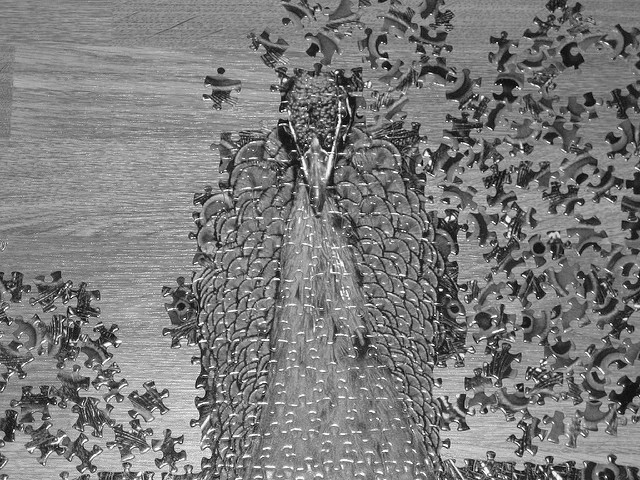
\includegraphics[width=0.7\paperwidth,height=0.7\paperheight,keepaspectratio]{PeacockPuzzleBW.jpg}

We actually exist in a state of \textit{thrownness}, of being \textit{thrown} into the world, where we don't have a choice about being here, can't control the flow of time, and are constantly adapting to the environment.
\newpage
This concept entered philosophy due to Martin Heidegger
  \begin{figure}[!htb]
        \center{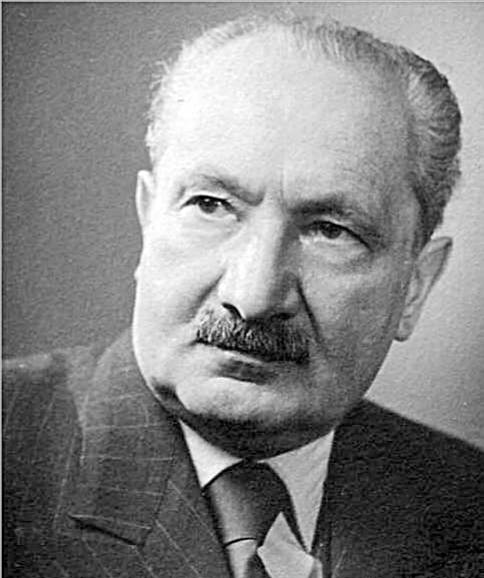
\includegraphics[width=0.5\paperwidth,height=0.5\paperheight,keepaspectratio]{Heidegger.jpg}}
        \caption{Martin Heidegger, total asshole}
\end{figure}
    
But he's an asshole and I'd rather not talk about him. Instead, I want to talk about Terry Winograd \& Fernando Flores's description of the idea from their book \textsc{Understanding Computers and Cognition}.

Imagine you're at a meeting. It could be at a job or planning a group project for a class or anything where multiple people need to come to some kind of conclusion or plan. Winograd \& Flores list some of the properties of this environment. Namely that
\begin{itemize}
    \item You have to do something. Even silence is an action that affects the other people around you
    \item The state of the system is constantly changing. Everyone is affecting everyone else every second that passes
    \item You're always \textit{interpreting} everyone else's actions. You don't know what every facial tic or tone of voice or word choice means, so you're making a choice about what it means
    \item Everyone else is interpreting you
    \item You're figuring out what the goal even is. The problem itself is changing over time
    \item Everyone's interpretations and actions are affected by all the previous experiences they've had
\end{itemize}

Okay, so what's this whole part about \textit{interpreting}? What if we had a magical telepathy machine so everyone could hear what everyone else is thinking, would that fix everything?

\textbf{No, actually!}

Why? Because we have finite processing power! Even if you had all the information about what everyone was thinking and all the historic context each person individually has you don't have the \textit{time} to try and understand it all. 

Time keeps marching on while you're trying to understand everything and, like we've already said, you have to do something. Even sitting and thinking counts as an action. There's no way to detach and deliberate like you would with a jigsaw puzzle. There's no way to know enough in advance that you're not making choices of interpretation to understand the world.
\newpage
\section{What's the point?}
So who cares? 

Well, think of \textit{thrownness} as a different way of looking at the world. It puts a lot of things into a different perspective. For example, what actual AI might look like, the problems with scientism and the goal of being ``perfectly rational'', or the way most self-help books assume your brain works like a computer you can program. 

\end{document}

